\chapter{Що таке відкриті дані?}

\subsection{Визначення відкритих даних}

\textbf{Відкриті дані (англ. Open Data)} – це концепція, яка відображає ідею, що визначені дані мають бути доступні для легкої обробки програмними засобами (machine readable) та подальшого використання і розповсюдження без жодних обмежень і контролю, в тому числі й для комерційного використання. Відкриті дані – це не просто інформація, а концепція, тобто система поглядів, підходів, процесів, які мають одну ідею та мету – вільного використання і розповсюдження даних про діяльність державних органів та органів місцевого самоврядування через мережу Інтернет.

Згідно загальноприйнятої в світі концепції, обов’язково безоплатними можуть бути тільки ті дані, які знаходяться у власності держави («ліцензійно чисті»), і якщо вони подаються в первинному необробленому вигляді. Додаткова обробка або доступ до API частіше за все лімітуються або коштують грошей. Крім того, хто завгодно може (з обов’язковим посиланням на джерело) використати дані в комерційний спосіб, створити на базі них власну програму чи обробити та надати нову цінність (розкласифікувати, встановити зв’язки тощо). Безумовно, всі витрати на додаткову роботу редакторів, програмістів та інше оплачує замовник (або кінцевий користувач).

Відкриті дані дозволяють повторно і необмежено використовувати інформацію, поєднувати її між собою, зменшити або виключити зайві витрати на дублювання та опрацювання великих масивів даних, реєстрів, довідників, баз даних тощо, створених в різних органах влади.

Закон "Про внесення змін до деяких законів України щодо доступу до публічної інформації у формі відкритих даних" №2171 від 19.02.2015 (прийнятий 09.04.2015) визначає наступний термін:

\begin{quote}
\textbf{Публічна інформація у формі відкритих даних} – це публічна інформація у форматі, що дозволяє її автоматизоване оброблення електронними засобами, вільний та безоплатний доступ до неї, а також її подальше використання.
\end{quote}

\subsection{Класифікація відкритих даних}

В законопроекті одночасно використовуються поняття «форма» та «формат», що не є тотожними. Розглянемо детально.

Для того, щоб зрозуміти, які можуть бути форми відкритих даних, ми також звернемося до відомої класифікації \textbf{«5 зірок Open Data»} (\url{http://5stardata.info/}), де якість даних та рівень відкритості визначається кількістю зірок від 1 до 5, чим більше – тим краще. Відкритість даних залежить від способів доступу, форматів та кількості додаткових дій, які потрібні для отримання кінцевої інформації, її обробки та збереження у власному сховищі або базі даних.

\begin{figure}[h]
    \centering
    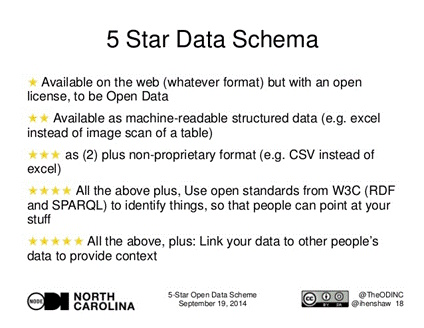
\includegraphics[width=\textwidth]{images/001.gif}
    \caption{5 зірок Open Data}
\end{figure}

\begin{itemize}
    \item \textbf{Одну зірку (*)} отримує будь-яка інформація, вільно доступна через Інтернет в будь-якому форматі. Під цю класифікацію підпадає файл у форматі PDF або інша (сканована) копія документу, на який веде пряме посилання на офіційному сайті державного органу.
    \item \textbf{Дві зірки (**)} отримує структурована інформація, яку можна обробляти автоматично, наприклад, у форматах для веб-браузерів чи офісних програм (відкриті формати – TXT, HTML, RSS; пропрієтарні формати, Excel – XLS, Word – DOC, RTF).
    \item \textbf{Три зірки (***)} може отримати інформація, представлена у відомих, добре описаних відкритих структурованих форматах (наприклад, CSV, JSON, XML, YAML).
    \item \textbf{Чотири зірки (****)} надаються у випадку, якщо можна отримати первинні необроблені набори відкритих даних у вигляді файлів або фільтровані дані у запиті до API за вказаними параметрами.
    \item \textbf{П’ять зірок (*****)} надається інформації, коли набори відкритих даних пов’язані між собою і представляють собою семантичну мережу.
\end{itemize}

\subsection{Формати даних}

В залежності від специфіки даних, їх розміру та тематики (геологія, тендери, реєстри, судові документи тощо), одні проекти відкритих даних створювались на базі наборів PDF чи DOC файлів, таблиць XLS, що перетворювались на прості текстові таблиці CSV, а інші брали за основу формат розмітки XML, проектували власні схеми XSD і використовували складні структури.

\subsubsection{Табличні формати}

\paragraph{CSV (Comma-Separated Values)}

CSV (від англ. \textit{Comma-Separated Values} – значення, що розділені комами) – текстовий відкритий формат, призначений для представлення таблиць (масивів, наборів) даних.

\begin{verbatim}
1997,Ford,E350,"ac, abs, moon",3000.00  
1999,Chevy,"Venture ""Extended Edition""","",4900.00  
1996,Jeep,Grand Cherokee,"MUST SELL! air, moon roof, loaded",4799.00  
\end{verbatim}

\paragraph{XLS/XLSX (Document Office Open XML)}

Файл XLSX - електронна таблиця, створена в Microsoft Excel - додатку для роботи з таблицями.

\subsubsection{Графічні формати}

\paragraph{JPEG (Joint Photographic Experts Group)}

JPEG (англ. \textit{Joint Photographic Experts Group}) - один з популярних графічних форматів, застосовуваний для зберігання фотозображень.

\paragraph{PNG (Portable Network Graphics)}

PNG (англ. \textit{Portable network graphics}) - растровий формат зберігання графічної інформації, що використовує стиснення без втрат.

\paragraph{TIFF (Tagged Image File Format)}

TIFF (англ. \textit{Tagged Image File Format}) - формат зберігання растрових графічних зображень.

\subsubsection{Текстові формати}

\paragraph{TXT (Textfile)}

TXT - це формат, що містить текстові дані, які, як правило, організовані у вигляді рядків.

\paragraph{Markdown}

Markdown - полегшена мова розмітки, створена з метою написання максимально читабельного і зручного для редагування тексту.

\subsubsection{Текстово-графічні формати}

\paragraph{HTML (HyperText Markup Language)}

HTML (від англ. \textit{HyperText Markup Language}) - стандартна мова розмітки документів у Всесвітній павутині.

\paragraph{DOCX (Document Office Open XML)}

DOCX (\textit{Document Office Open XML}) - формат файлу для зберігання електронних документів пакетів офісних додатків.

\paragraph{OpenDocument format (LibreOffice/OpenOffice)}

Формат OpenDocument - це формат для текстових, табличних документів та презентацій.

\paragraph{PDF (Portable Document Format)}

Формат переносного документа (PDF) - це формат файлу, який використовується для надійного уявлення і обміну документами.

\subsubsection{Формати представлення даних через API}

\paragraph{JSON (JavaScript Object Notation)}

JSON (від англ. \textit{JavaScript Object Notation}) – текстовий відкритий формат, оснований на Javascript представлені.

\begin{verbatim}
{
    "firstName": "Иван",
    "lastName": "Иванов",
    "address": {
        "streetAddress": "Московское ш., 101, кв.101",
        "city": "Ленинград",
        "postalCode": 101101
    },
    "phoneNumbers": [
        "812 123-1234",
        "916 123-4567"
    ]
}
\end{verbatim}

\paragraph{XML (eXtensible Markup Language)}

XML (від англ. \textit{eXtensible Markup Language}) – мова розмітки, що розширюється.

\begin{verbatim}
<person firstName="Иван" lastName="Иванов">
    <address streetAddress="Московское ш., 101, кв.101"
        city="Ленинград" postalCode="101101"/>
    <phoneNumbers>
        <phoneNumber>812 123-1234</phoneNumber>
        <phoneNumber>916 123-4567</phoneNumber>
    </phoneNumbers>
</person>
\end{verbatim}

\subsubsection{Формати даних для роботи з геопросторовими даними}

\paragraph{GeoJSON та TopoJSON}

GeoJSON - відкритий формат, призначений для зберігання графічних структур даних.

\begin{verbatim}
{
    "type": "FeatureCollection",
    "features": [
        {
            "type": "Feature",
            "geometry": {"type": "Point", "coordinates": [102.0, 0.5]},
            "properties": {"prop0": "value0"}
        },
        {
            "type": "Feature",
            "geometry": {
                "type": "LineString",
                "coordinates": [
                    [102.0, 0.0], [103.0, 1.0], [104.0, 0.0], [105.0, 1.0]
                ]
            },
            "properties": {
                "prop0": "value0",
                "prop1": 0.0
            }
        },
        {
            "type": "Feature",
            "geometry": {
                "type": "Polygon",
                "coordinates": [
                    [ [100.0, 0.0], [101.0, 0.0], [101.0, 1.0],
                        [100.0, 1.0], [100.0, 0.0] ]
                ]
            },
            "properties": {
                "prop0": "value0",
                "prop1": {"this": "that"}
            }
        }
    ]
}
\end{verbatim}
